\chapter{Wyniki} \label{chap:outcomes}

\section{Wstęp}

W celu zbadania działania systemu przeprowadzone zostały następujące pomiary:

\begin{itemize}
\item pomiar czasu wykonania programu w zależności od liczby samochodów na skrzyżowaniu 
\item pomiar ilości korków czasowych po których wszystkie samochody opuszczą skrzyżowania w zależnośći od liczby samochodów na skrzżowaniu
\end{itemize}

Pomiary zostały wykonane na dwóch sieciach dróg:
\begin{itemize}
\item skrzyżowanie ze sobą ośmiu dróg
\item skrzyżowanie ze sobą czterech dróg
\end{itemize}

Drogi na obydwu sieciach mają rozmiar 24.
\newline
\newline
Reprezentacja graficzna skrzyżowań jest przedstawiona na rysunkach \ref{eight-roads-crossroads} oraz \ref{four-roads-crossroads} z przykładowymi rozmieszczeniami pojazdów.
\begin{figure}
    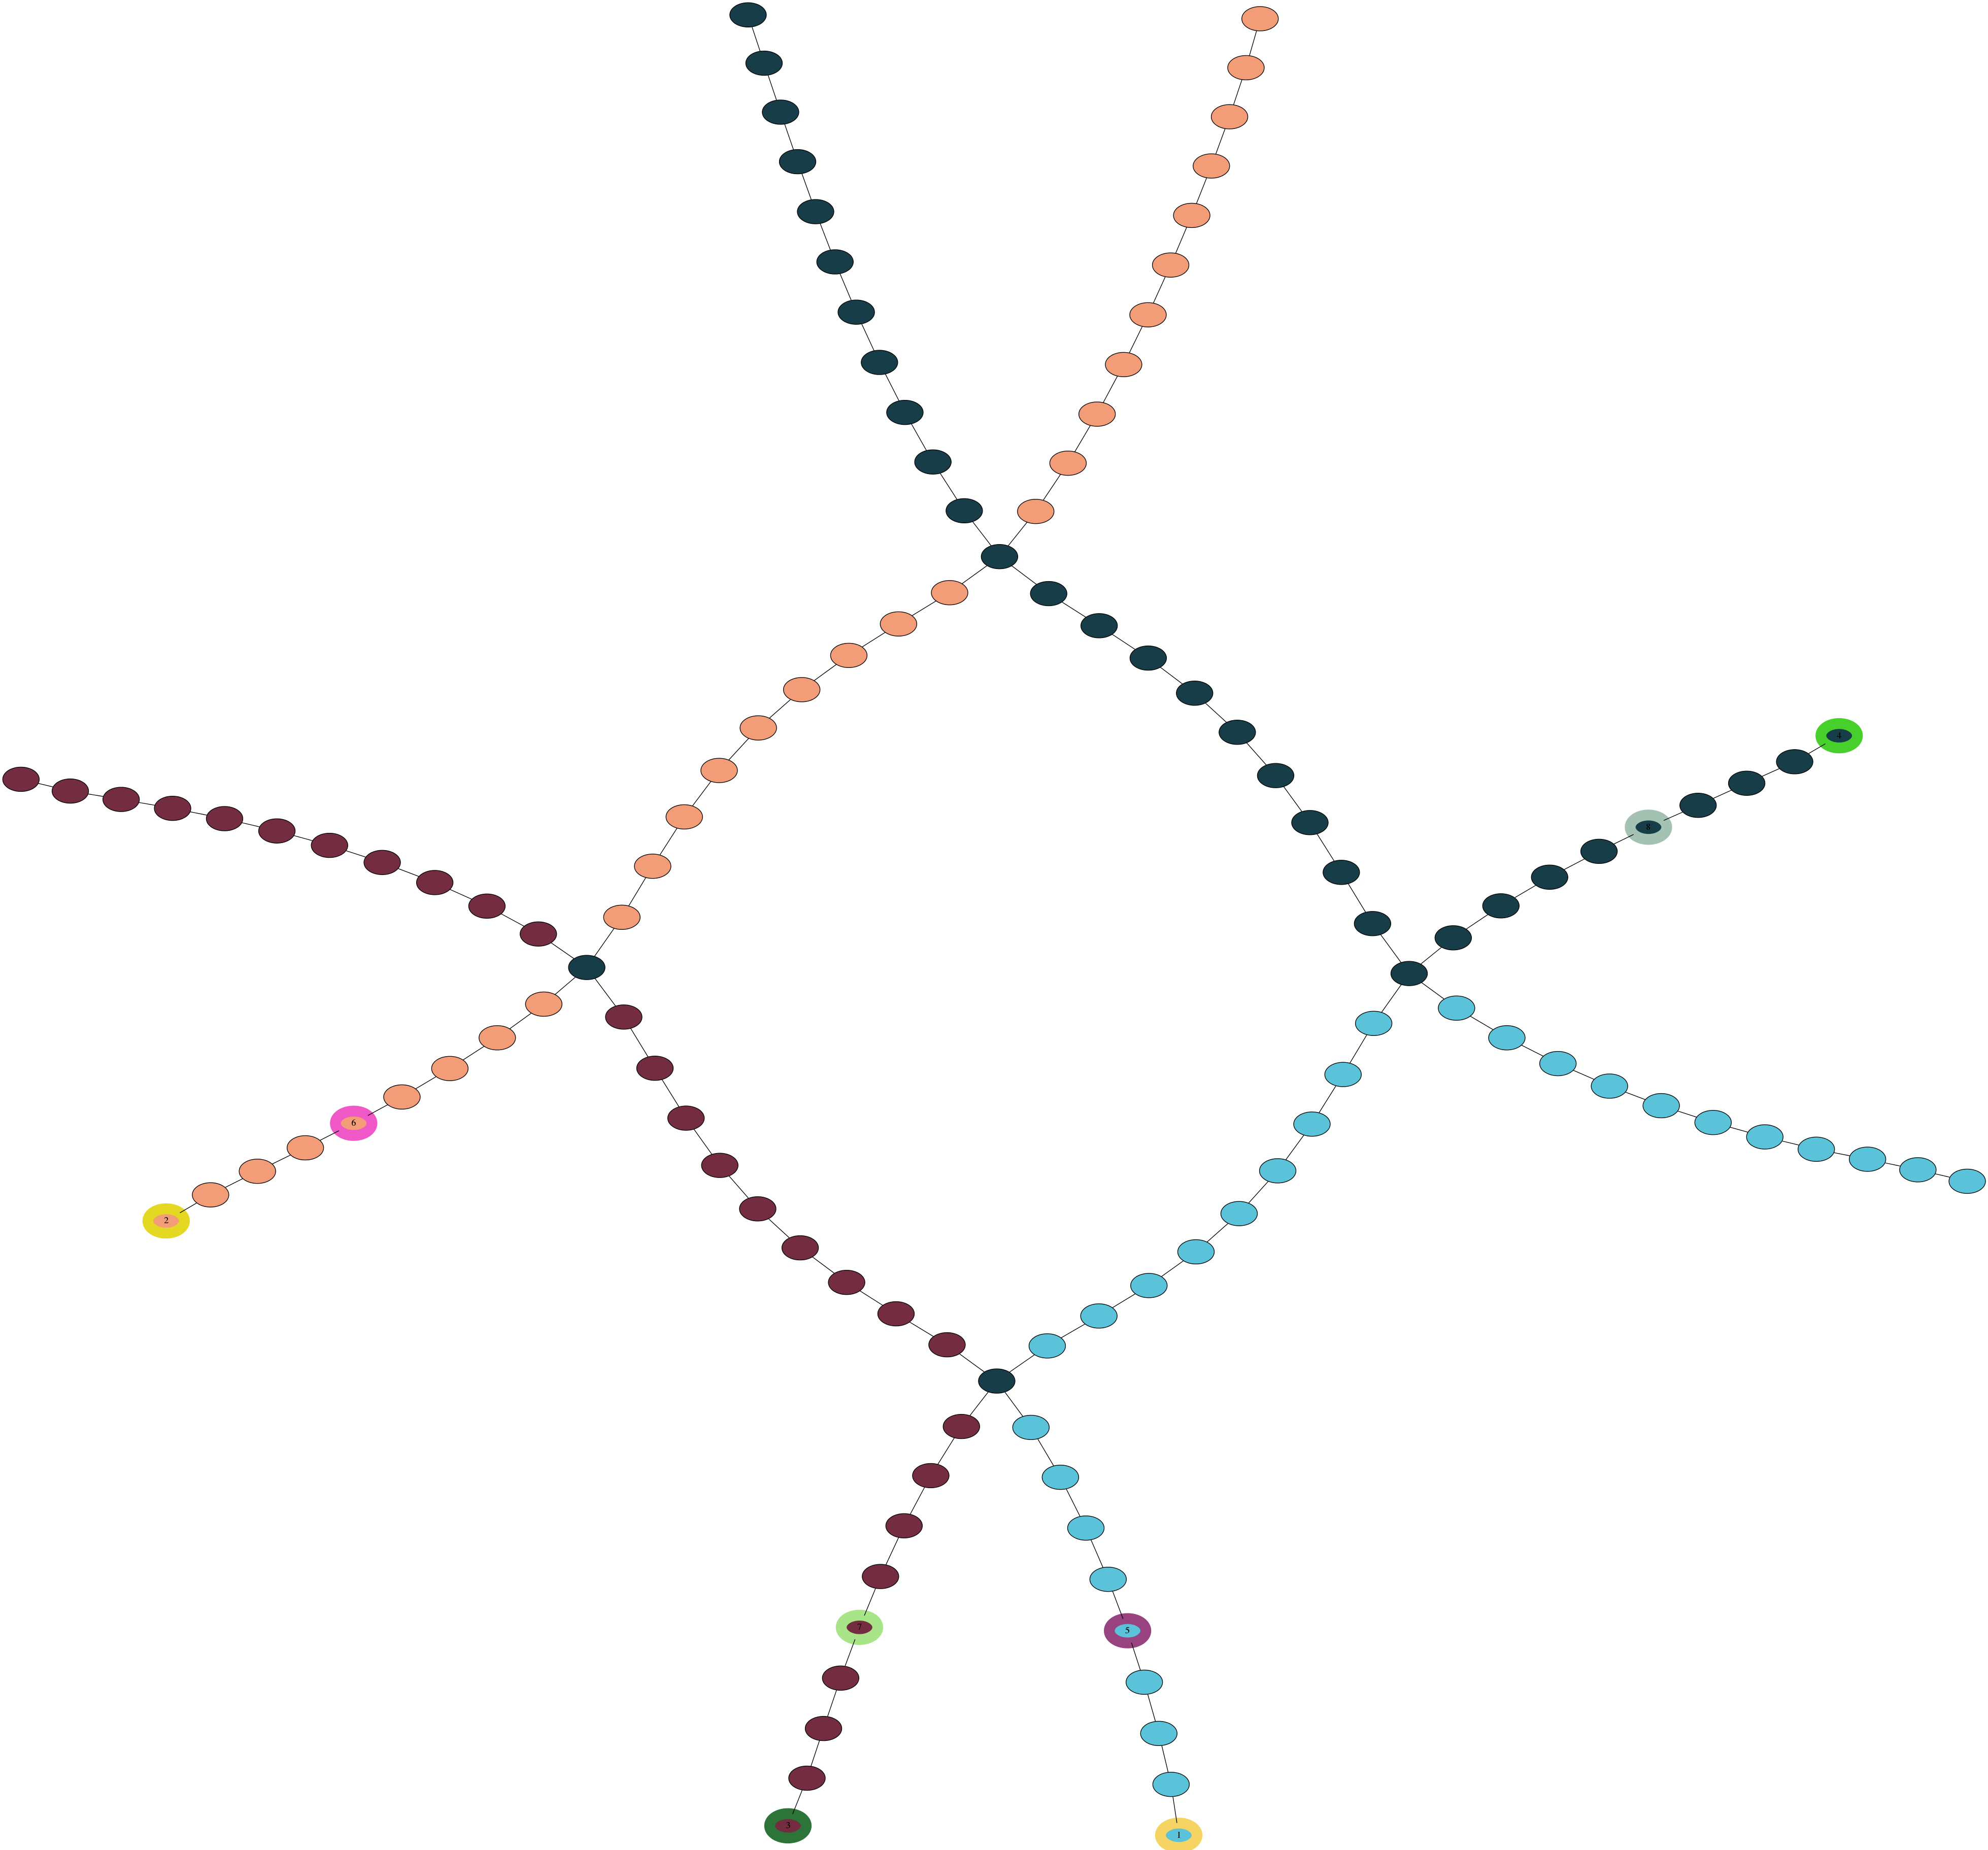
\includegraphics[width=1.0\textwidth]{1.png}
  \caption{Skrzyżowanie ośmiu dróg}
  \label{eight-roads-crossroads}
\end{figure}
\begin{figure}
    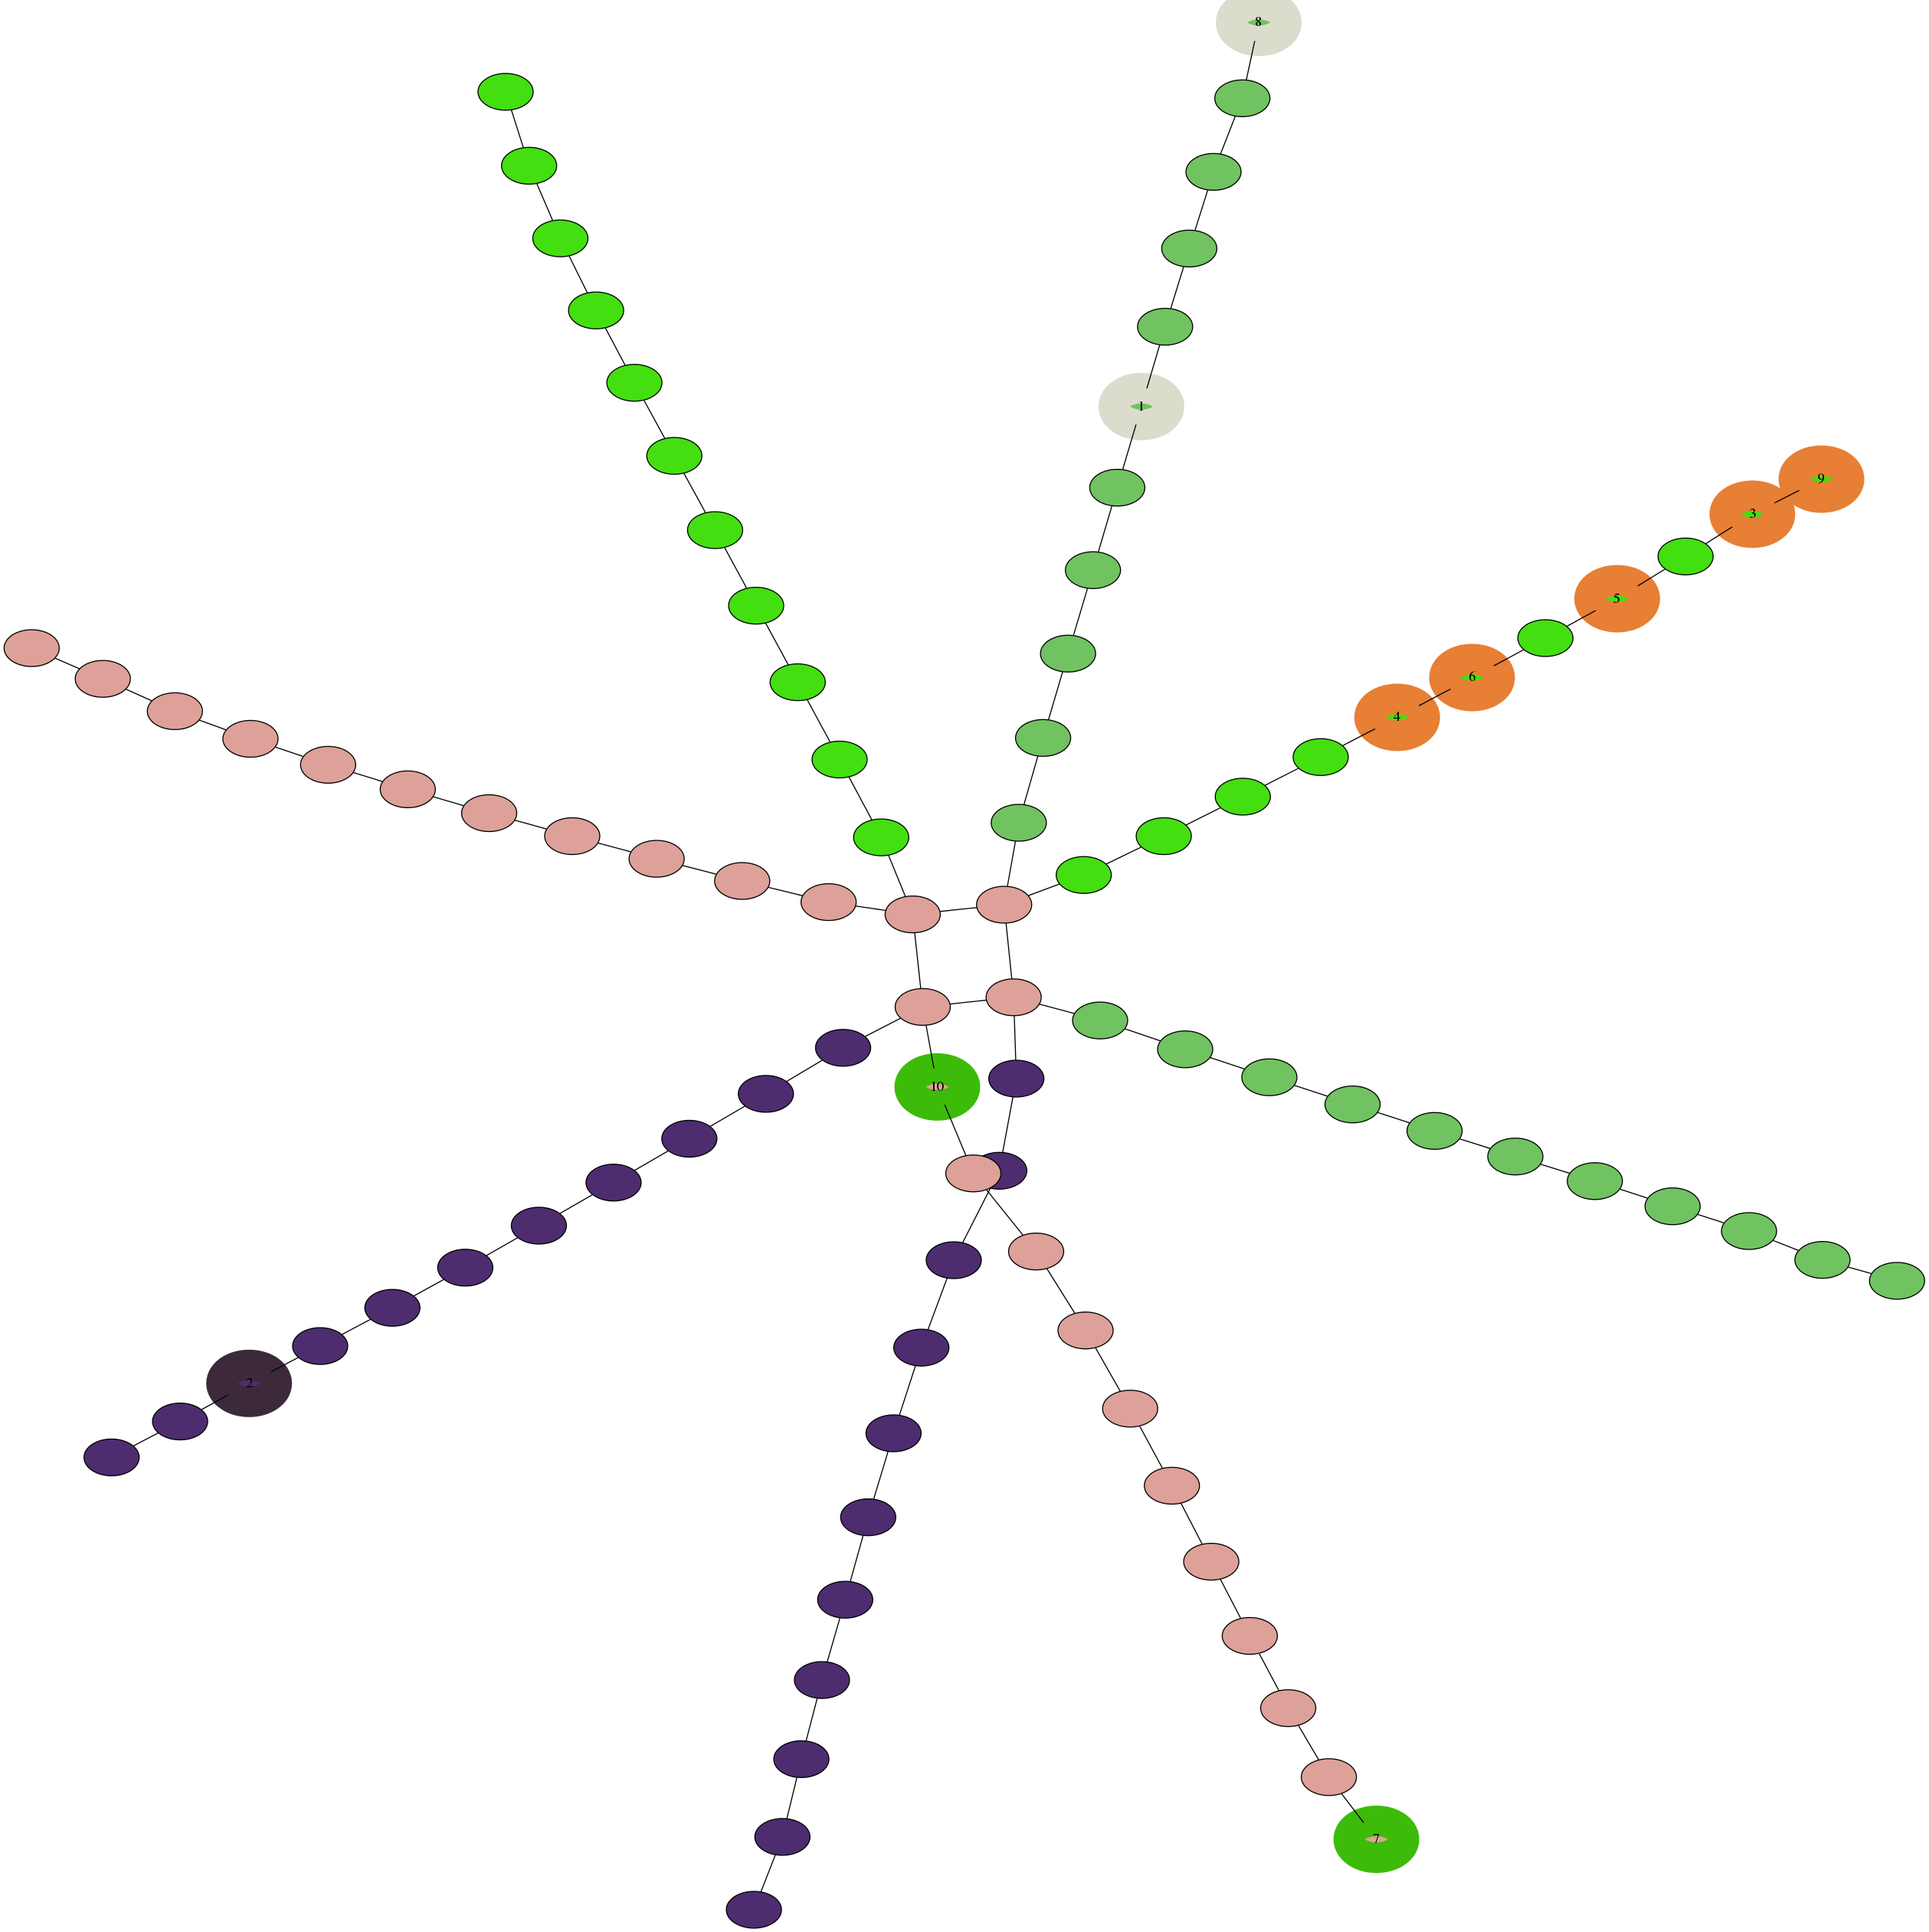
\includegraphics[width=1.0\textwidth]{4_roads.png}
  \caption{Skrzyżowanie czterech dróg}
  \label{four-roads-crossroads}
\end{figure}

Pomiary zostały przeprowadzone dla następującej liczby samochodów \{2, 4, 6, 8, 10, 12\}.
\newline
\newline
Dla każdej liczby samochodów wygenerowane losowo zostało 30 położeń pojazdów przy założeniu, że żaden z pojazdów nie startuje za ostatnim skrzyżowaniem.

\section{Wyniki pomiarów dla skrzyżowania czterech dróg}

Zgodnie z wcześniej opisanymi założeniami dla skrzyżowania czterech dróg program został uruchomiony 30 razy dla samochodów ze zbioru \{2, 4, 6, 8, 10, 12\} co razem daje 180 uruchomień.
\newline
\newline
Wykresy przedstawiające wyniki na skrzyżowaniu czterech dróg zaprezentowane są na rysunkach \ref{four-roads-crossroads-execution-time} oraz \ref{four-roads-crossroads-timesteps}
\begin{figure}[ht]
  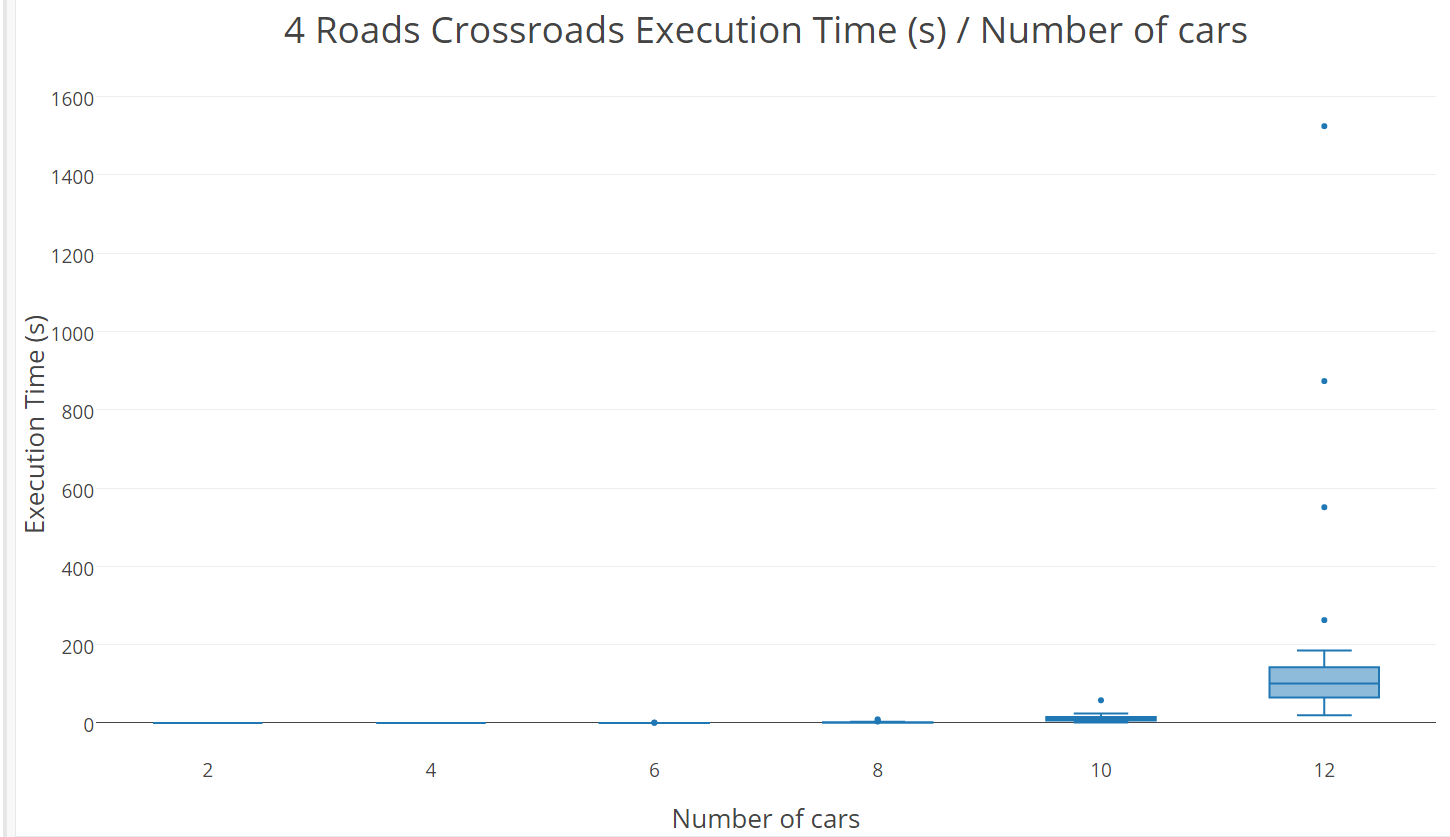
\includegraphics[width=1.0\textwidth]{4_roads_crossroads_execution_time_2.png}
  \caption{Wykres zależności czasu wykonania programu od liczby pojazdów}
  \label{four-roads-crossroads-execution-time}
\end{figure}
\begin{figure}[ht]
  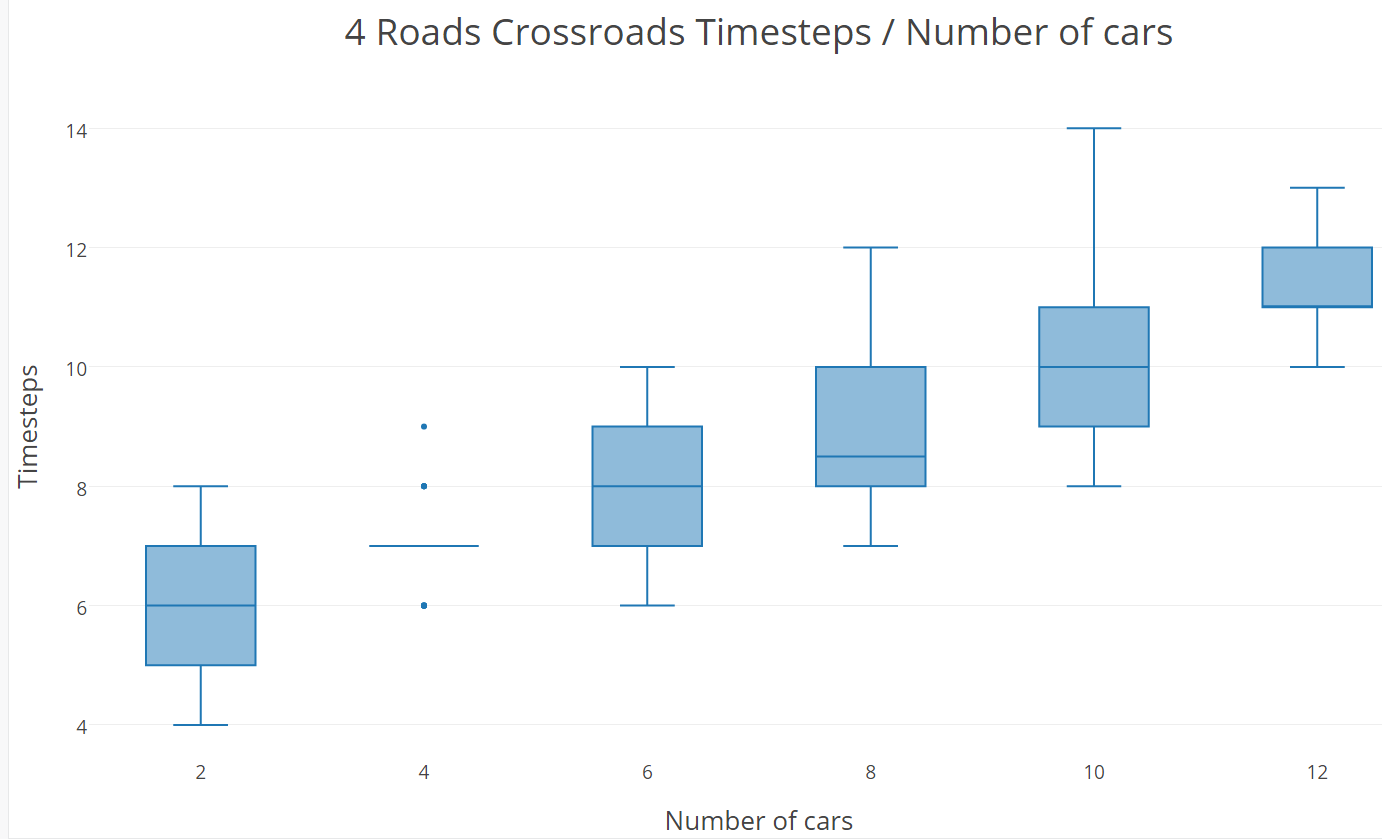
\includegraphics[width=1.0\textwidth]{4_roads_timesteps_2.png}
  \caption{Wykres zależności kroków czasowych od liczby pojazdów}
  \label{four-roads-crossroads-timesteps}
\end{figure}

\section{Wyniki pomiarów dla skrzyżowania ośmiu dróg}

Dla skrzyżowania ośmiu dróg też zostało przeprowadzone 180 uruchomień.
\newline
\newline
Wykresy przedstawiające wyniki na skrzyżowaniu czterech dróg zaprezentowane są na rysunkach \ref{four-roads-crossroads-execution-time} oraz \ref{four-roads-crossroads-timesteps}
\begin{figure}[H]
    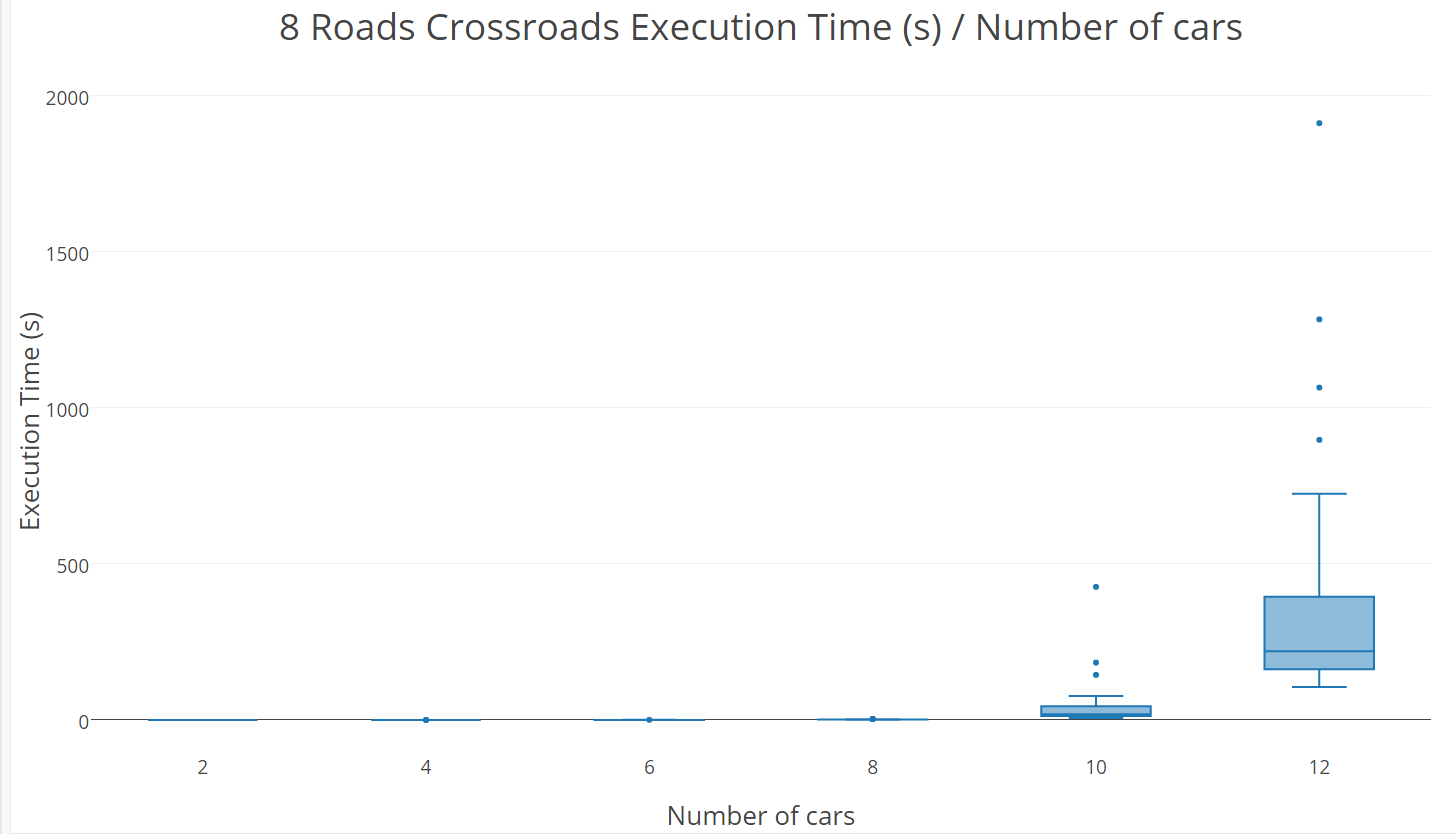
\includegraphics[width=1.0\textwidth]{8_roads_execution_time_2.png}
  \caption{Wykres zależności czasu wykonania programu od liczby pojazdów}
  \label{eight-roads-crossroads-execution-time}
\end{figure}
\begin{figure}[H]
    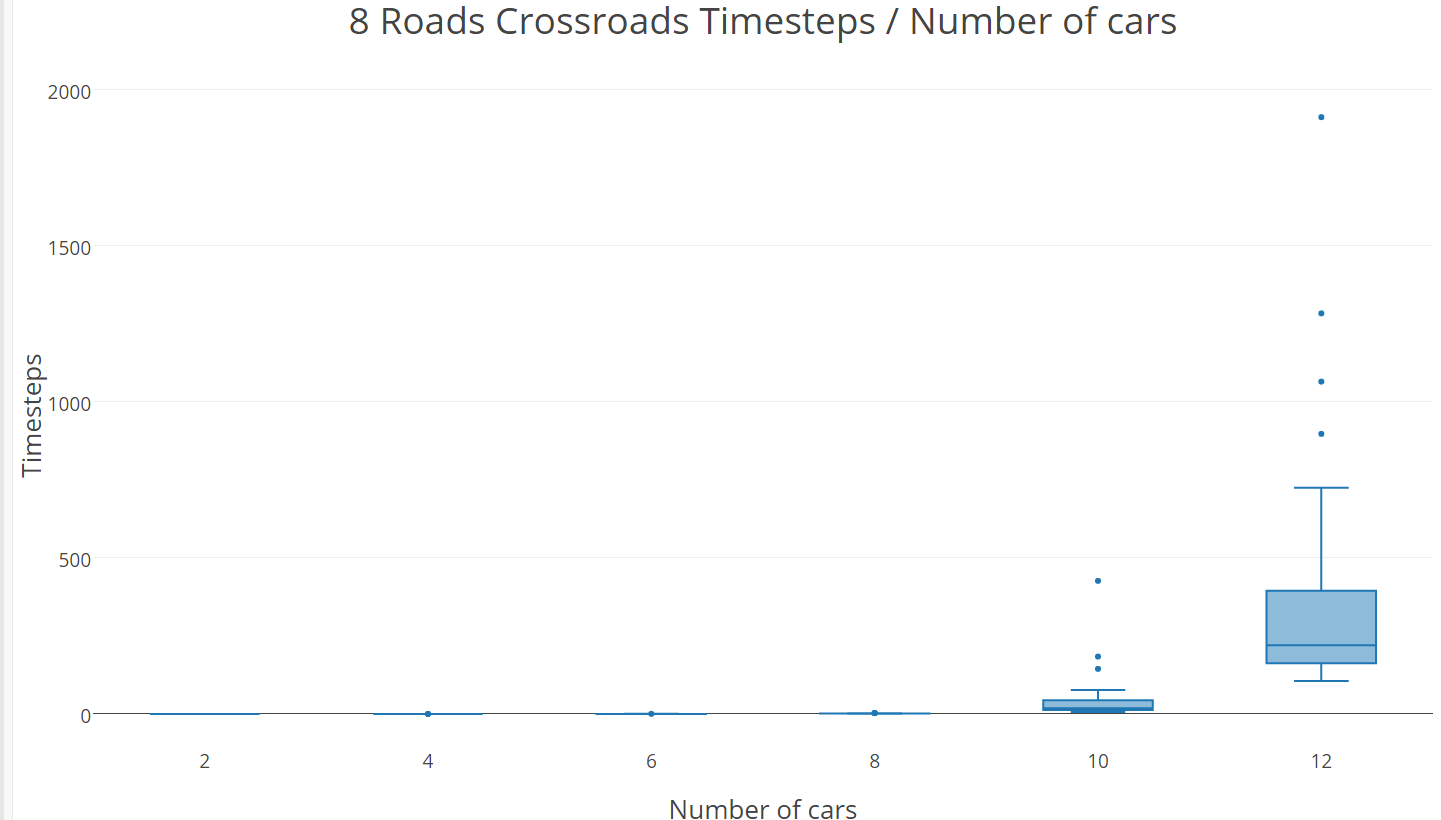
\includegraphics[width=1.0\textwidth]{8_roads_timesteps_2.png}
  \caption{Wykres zależności kroków czasowych od liczby pojazdów}
  \label{eight-roads-crossroads-timesteps}
\end{figure}

\section{Porównanie wyników z rozwiązaniem ze światłami drogowymi}

W celu zweryfikowania szybkości podejścia z wykorzystaniem zmodyfikowanej wersji A* pomiary zostały porównane z rozwiązaniem polegającym na optymalizacji świateł drogowych przedstawionym w pracy [TUTAJ CYTAT PRACY SEBASTIANA].
\newline
\newline
Wykonując pomiary uzgodnione zostały wspólne warunki w obu rozwiązanich tak, aby można było w krokach czasowych porównać oba rozwiązania.
\newline
\newline
Wykres z wynikami pokazany jest na rysunku \ref{comparison}
\begin{figure}[ht]
  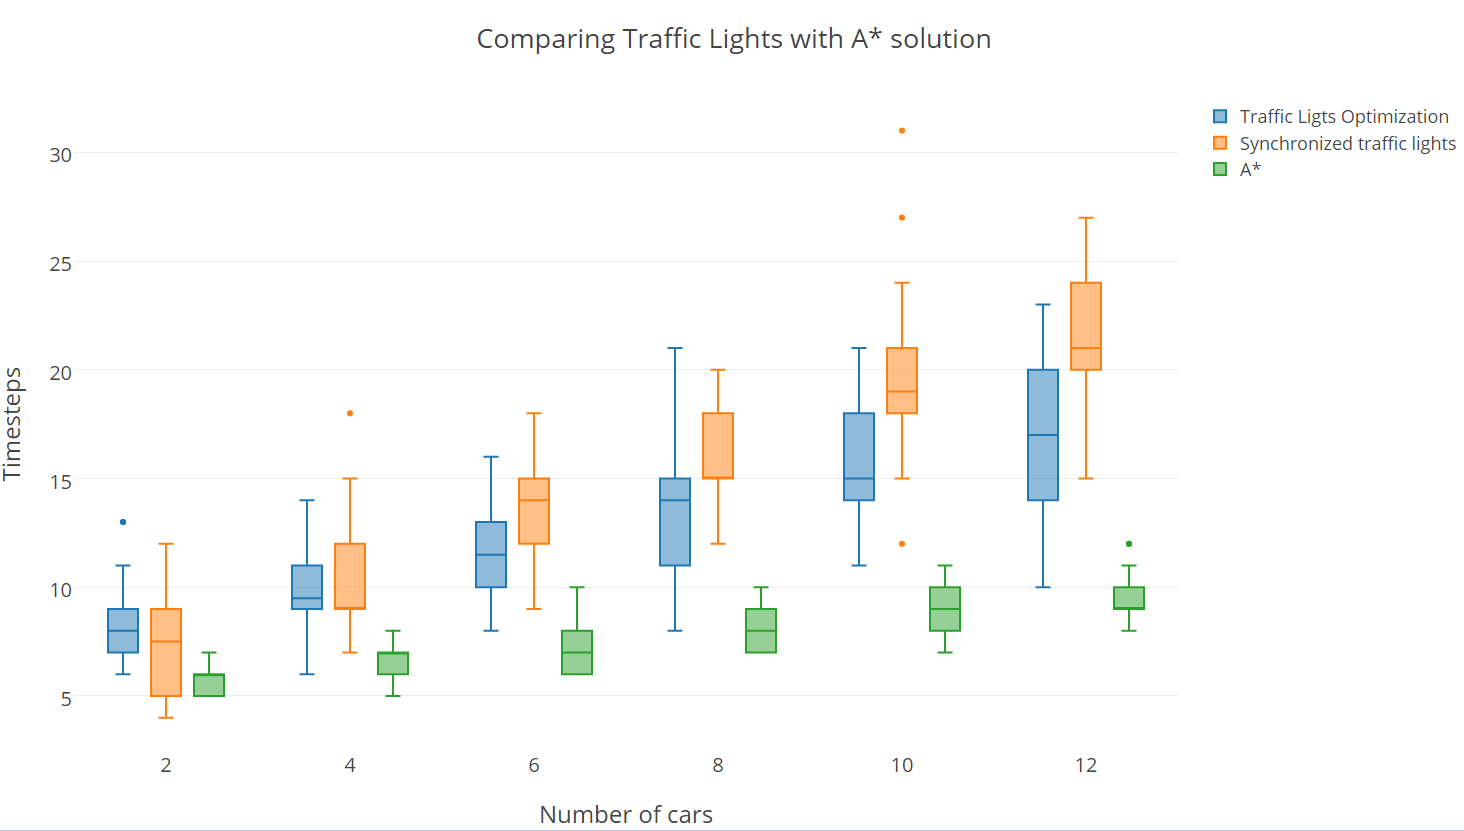
\includegraphics[width=1.0\textwidth]{8_roads_comparison_2.png}
  \caption{Porównanie rozwiązania ze zmodyfikowanym A* z zoptymalizowanymi światłami drogowymi na skrzyżowaniu ośmiu dróg}
  \label{comparison}
\end{figure}
